\documentclass{article}
\usepackage[utf8]{inputenc}
\usepackage{hyperref}
\usepackage{url}
\usepackage{mathtools}
\usepackage{amsmath}
\usepackage{graphicx}
\usepackage{wrapfig}
\usepackage{algorithm}
\usepackage{algpseudocode}
\usepackage{subcaption}
\usepackage[svgnames]{xcolor}
\usepackage{listings}
\usepackage[left=2.5cm, right=2.5cm, top=1.5cm, bottom=2cm]{geometry}
\setcounter{section}{-1}
\setlength\parindent{0pt}

\title{
\textbf{Algorithmics for Data Mining: Deliverable 1\\} \Large{
    Handwitten images classificator}}
\author{Oriol Borrell\\
\textit{\small FIB - UPC Student} \\
\textit{\small Barcelona, Spain} \\
\textit{\texttt{\href{mailto:oriol.borrell.roig@est.fib.upc.edu}
{\small oriol.borrell.roig@est.fib.upc.edu}}}}
\date{\today}

\begin{document}
\maketitle

\section{Abstract}
\textit{
In this project we have trained a model\cite{CODE} in order to classify handwritten images within a given categories. In this essay we will focus on the main CRISP-CM methodology steps that were taken into account when developing the project, while showing and explaining the obtained results.
}

\section{Problem Understanding}
In this project we will define two different types of goals: The problem goal and the data mining goal. The data mining goal is clear: perform a model that let us classify a drawing in one of the given categories. We will consider acceptable a model with an accuracy bigger than 0.5.

Although the data mining is a very important part of the project, being able to predict the category with a certain accuracy is not the main goal of the project. The principal objective is to practice with the CRISP-DM methodology and understand it's main characteristics. The performance of this article will be proof of success.

\section{Data Understanding}
The data used will be obtained from the Quick Draw\cite{QDP} project, by Google. This dataset has millions of drawings organized in the different categories that each represent. This is an open source dataset create by Google, Inc. under the Creative Commons Attribution 4.0 International license\cite{QDL} so there are no legal problems when using this data.

The data is downloaded from the Google Cloud Platform\cite{GCP}. The original dataset contains around 50 million hand-written drawings classified in 345 categories depending on what the drawing represents. When defining the project to the teacher we accord to use for this first delivery only 2 categories, with aproximately 10.000 drawings each.

\subsection{Data Description}
\label{sec:Data_Description}
The data for each category is downloaded separately. The data is stored in \textit{.ndjson} file, where each row represents a drawing. Each drawing contains the following information:
\begin{itemize}
    \setlength\itemsep{0.05em}
    \item \textbf{Key\_id:} A unique identifier across all drawings
    \item \textbf{Word:} Category the player was prompted to draw. In our project, this attribute can only have the following 2 values: ambulance or angel.
    \item \textbf{Countrycode:} A two letter country code of where the player was located.
    \item \textbf{Timestamp:} When the drawing was created.
    \item \textbf{Recognized:} Boolean representing whether the word was recognized by the game.
    \item \textbf{Drawing:}  A JSON array representing the vector drawing, represented with strokes.
\end{itemize}

\subsection{Data Exploration}
In the original dataset, each category contained around 100.000 drawings. As we will use much less than that, whe had to select the data we will us to train and test the model. This selection criteria is explained in Section \ref{sec:Data_Preparation}: Data Preparation.

Once we had our data, the first thing I did is to try to understand how data is distributed for \textit{Word}, and \textit{Countrycode} attributes. In Figure \ref{fig:Category-Attribute} is shown the number of appearances of each category. In Figure \ref{fig:Countrycodes-Attribute} the percentage of countries where the draw was made. It's important to mention that the 'Others' section in Figure \ref{fig:Countrycodes-Attribute} is composed by 99 countries where its percentage is no grader than 1\%.

\begin{figure}[H]
    \centering
    \begin{subfigure}{.45\textwidth}
      \centering
      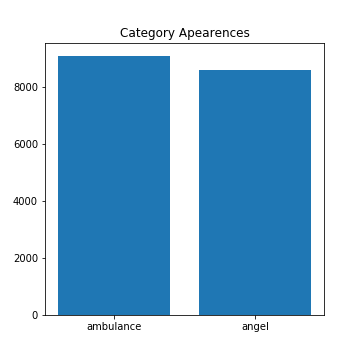
\includegraphics[width=.95\textwidth]{./img/Category.png}
      \caption{Category Attribute.}
      \label{fig:Category-Attribute}
    \end{subfigure}
    \begin{subfigure}{.45\textwidth}
        \centering
        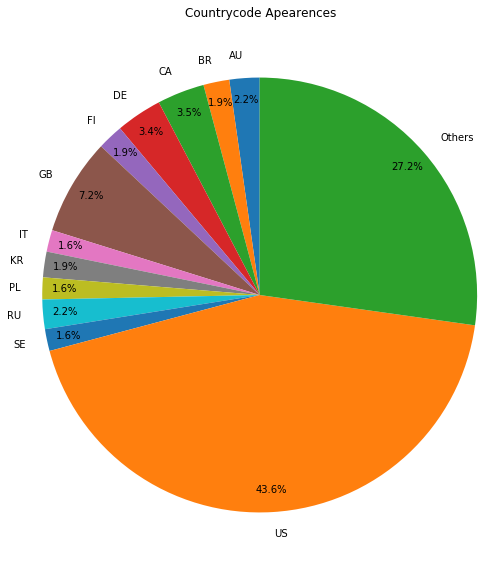
\includegraphics[width=0.95\textwidth]{./img/Country.png}
        \caption{Countrycodes Attribute.}
        \label{fig:Countrycodes-Attribute}
    \end{subfigure}
    \caption{Data Exploration}
    \label{fig:PCA}
\end{figure}
In Figure \ref{fig:Category-Attribute} we can appreciate that we have a balanced dataset. We cannot conclude the same in Figure \ref{fig:Countrycodes-Attribute}. We can see that most of the drawings are made in USA (43.6\%), being followed by GB (7.2\%). If we find that there's a correlation between the country code and the way people draw, this unbalance could affect to our model. For simplification of the problem we will suppose there's no correlation. About completeness of the data, we found that there are no nulls in the whole dataset. Moreover, each column has all the data in a correct format.

\subsection{Visualitzation}
In order to better understand the drawings we performed a Principal Component Analysis (PCA). PCA is an unsupervised learning algorithm as it ignores the class labels (the so-called principal components) that maximize the variance in a dataset, to find the directions.

In the first iteration we obtained the Figure \ref{fig:PCA_outliers}. The only conclusion possible was that we had some outliers that could make decrease the accuracy of our model. We deleted those drawings in section \ref{sec:Data_Selection}: Data Selection.

After removing those outliers we obtained Figure \ref{fig:PCA_no_outliers}. In this image we can clearly identify both classes: The yellow one represents the $angel$ category, and its located in the positive side of the first principal component. In the negative side of the first principal component we have the $ambulance$ images. Also, we observe that the $ambulance$ is more disperse than $angel$, and this could mean more variability in the drawings.

\begin{figure}[H]
    \centering
    \begin{subfigure}{.49\textwidth}
      \centering
      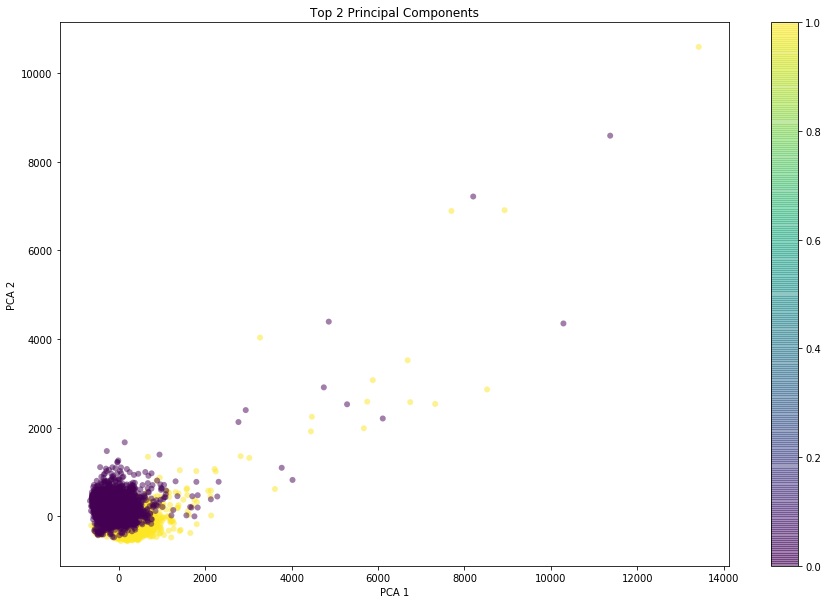
\includegraphics[width=1\textwidth]{./img/PCA_outliers.png}
      \caption{PCA with outliers.}
      \label{fig:PCA_outliers}
    \end{subfigure}
    \begin{subfigure}{.49\textwidth}
        \centering
        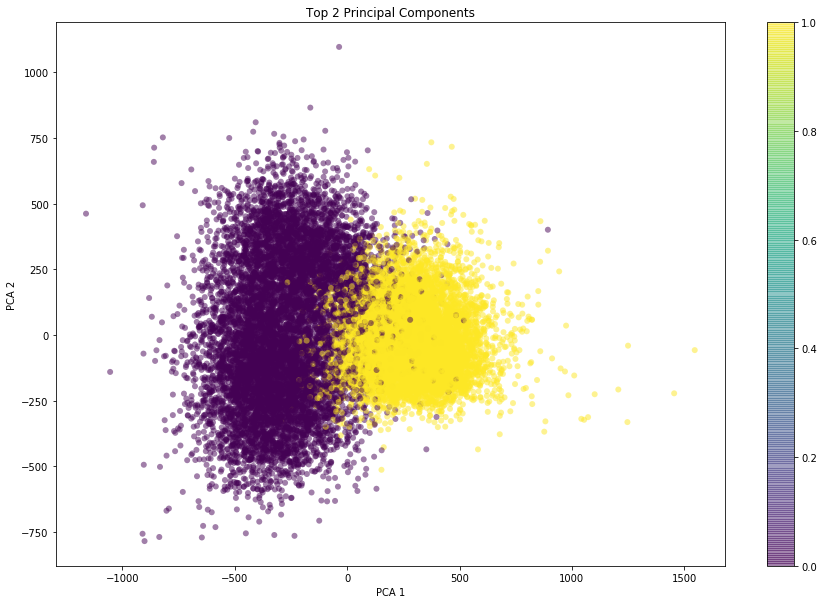
\includegraphics[width=1\textwidth]{./img/PCA_no_outliers.png}
        \caption{PCA without outliers.}
        \label{fig:PCA_no_outliers}
    \end{subfigure}
    \caption{Principal Component Analysis.}
    \label{fig:PCA}
\end{figure}

\section{Data Preparation}
\label{sec:Data_Preparation}
As we commented previously, the original dataset had no null values and mostly all the values were in a correct format. In this section we mainly focused in solving two problems: Selecting the data that we will use in the project, and converting the Drawing JSON array into an array in order to apply different models.

\subsection{Data Selection}
\label{sec:Data_Selection}
The main problem we had is that the original dataset contained a huge amount of data, that could not be computed in a reasonable time. To solve this problem we simplified the problem reducing the number of categories. As mentioned  in Section \ref{sec:Data_Description}, we selected the following ones: $ambulance$ and $angel$.

For this categories we downloaded the whole dataset, and created a script that selected randomly around 10.000 each. Those categories that had more rows in the original dataset will have more rows in ours.

The second problem we faced was that once performed the PCA, we realized we had some outliers that we wanted to erase. In order to delete them, we modified the selection script, including that all the rows selected must be recognized by the Google's algorithm (recognized attribute is \textit{True}). We are aware that this is not the best solution. It's the one that was accorded with the teacher in order to avoid too much complexity for this first deliverable. Detecting outliers could be the scope for future deliveries.

\subsection{Data Formating}
\label{sec:Data_Formating}
We performed two main changes with respect the original database. The easiest one was to convert the \textit{Word} attribute into numeric. The second change was to transform the JSON array for the images into a array that could be computed.

In order to do so, the plotted each image and save it as a \textit{.png} of size $150 \times 100$ pixels. We reduced that much the image for space and computation limitations. Once we had the image we transform it into a bitmap. Finally we transformed each bitmap into an array where each value represents the grey-scale value of the pixel, as the model requires.

\section{Modeling} 
\label{Modeling}
Once we had the data ready we applied our model: $k$-NN\cite{KNN}. Before applying any model we divided our data into train and test data (75\% - 25\%). To validate our models, we randomly selected 448 new rows in the original dataset for each category and applied them the same preprocessing steps mentioned previously.

The $k$-NN ($k$-Nearest Neighbors) algorithm applies a really simple idea: the algorithm classifies each new sample in the corresponding group, according to $k$ neighbors closer to one group or another. It calculates the distance of the new element to each of the existing ones, and orders those distances from least to greatest to select the group to which they belong.

The first thing we did is to find the $k$ that give us a better accuracy. We tried all the odd values from $1$ to $30$. Table \ref{tab:knn_results} shows the obtained values:

\begin{table}[ht]
    \centering
    \begin{tabular}{|l|l|l|}
        \hline
        \textbf{k} & \textbf{accuracy}  \\
        \hline
        1 & 55.16\% \\
        \hline
        3 & 51.89\% \\
        \hline
        5 & 52.02\% \\
        \hline
        7 & 53.18\% \\
        \hline
        \textbf{9} & \textbf{81.88\%} \\
        \hline
        11 & 81.42\% \\
        \hline
        13 & 79.12\% \\
        \hline
        15 & 77.79\% \\
        \hline
        17 & 75.55\% \\
        \hline
        19 & 74.89\% \\
        \hline
        21 & 73.94\% \\
        \hline
        23 & 72.79\% \\
        \hline
        25 & 71.77\% \\
        \hline
        27 & 71.23\% \\
        \hline
        29 & 70.98\% \\
        \hline
    \end{tabular}
    \caption{Accuracy obtained respect $k$}
    \label{tab:knn_results}
\end{table}

As the higher accuracy was obtained with $k=9$, we used this value to build our model. We re-trained the classifier and tried to predict the drawings that we reserved for validation. We got an accuracy of \textbf{0.710}. Taking into account that trying to predict the category randomly we would had an accuracy of 0.500, is an improvement, but not the improvement that we expected. In futures deliverables we could search for a model that works better with images, like Convolutional Neural Network (CNN).

\section{Evaluation}

The results obtained gave us an improvement comparing it with "flipping a coin" to predict the category. However, the accuracy obtained is not the one that we expected. As we mentioned this could be mainly for two reasons: The first one is that we find a god way to detect outliers, but it can be improved. The second one is because $k$-NN is not the best model to treat with images. This two points can be solved in future deliverables.

We have to take into account that obtaining a high accuracy was not the main goal of the project. In this essay we described all the important things we have taken into account in order to build a classifier for each phase of the CRISP methodology. We discussed from the legality to use the data, to the characteristics of the model, going through our considerations in data understanding and data preprocessing, for example. The discussion of each step and, after iterating several times in the methodology, we can affirm that our level is much more higher than it was. We set a good basis to work in future deliverables, explaining the things that could be improved in future steps. With the completion of this essay we conclude the main objective of this first deliverable.

\bibliography{references}{}
\bibliographystyle{unsrt}

\end{document}
